\textbf{Traduce el siguiente modelo Entidad – Relación a su correspondiente Modelo Relacional:}\vspace{.3cm}

\begin{center}
    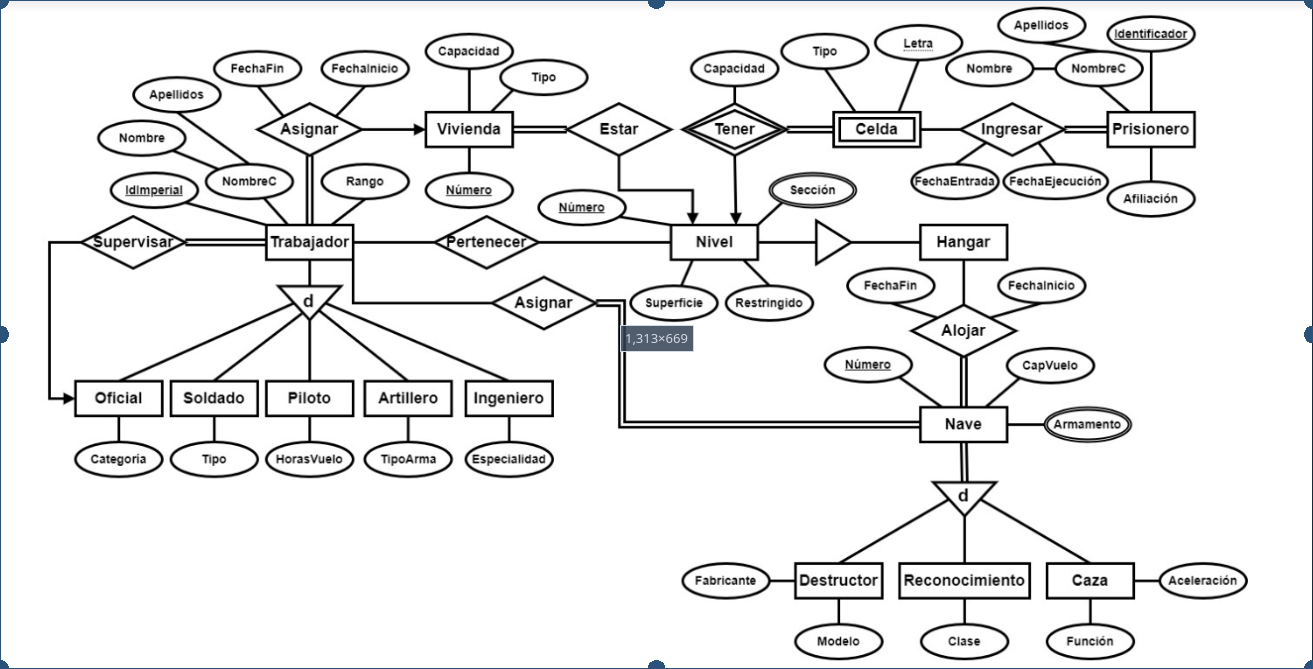
\includegraphics[width=12cm]{conversion/../resources/a.png}
\end{center}

Tras traducir, nos queda el siguiente modelo relacional:\vspace{.3cm}
\begin{center}
    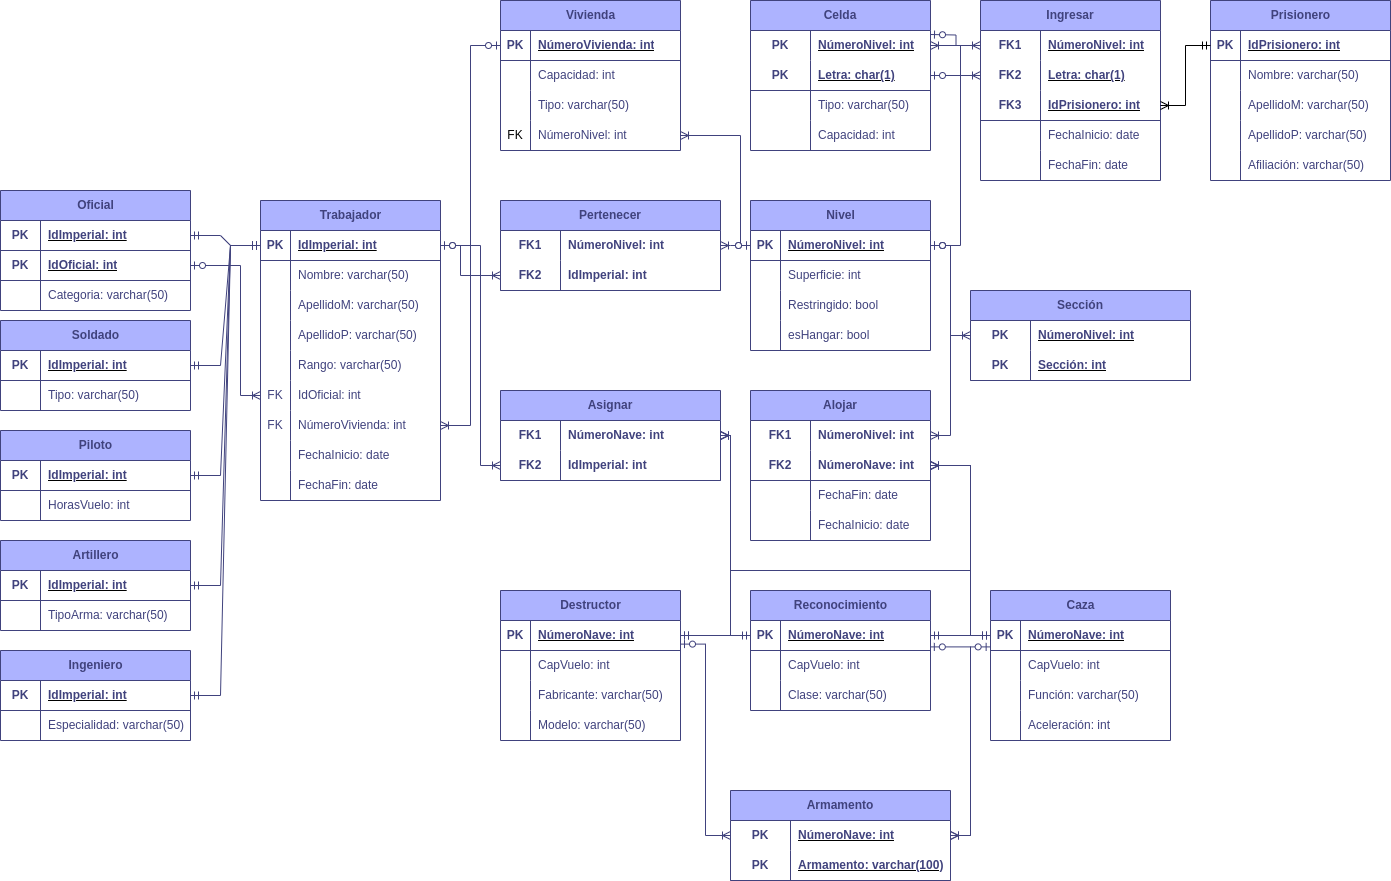
\includegraphics[width=12cm]{conversion/../resources/Tarea3.2.a.png}
\end{center}

La verdad es que hay varias que son tanto PK como FK pero me comentaron que
no era correcto ponerlas como PK y FK a la vez, así que seguí el pdf. \vspace{.2cm}

Para la parte de \textbf{Supervisar} entre Trabajador y Oficial, tuve que agregarle un
atributo \textbf{IdOficial} a la tabla Trabajador, ya que si no era guardar en Trabajador
un atributo IdTrabajador que no se entiende tanto y se pierde la semántica de la relación.\vspace{.2cm}

Ademas de esto, varias relaciones son del mismo tipo entonces sus conexiones se sobrelapan
lo que hace un poco difícil seguir el diagrama pero por lo demás, creo que está bien.\vspace{.2cm}

Finalmente, parti los \textbf{Apellidos} en \textbf{ApellidoP} y \textbf{ApellidoM} para que sea atomico.\vspace{.4cm}